% !TeX root = ../tesis.tex


\chapter{Reconstrucción con SSKK}

\label{section:apendix2}

En la Sección \ref{section:optical_properties} se reconstruyó la parte real de la función dieléctrica de los eritrocitos y del plasma mediante la aplicación de las relaciones SSKK. En esta sección se ilustra y discute dicha reconstrucción. En la Fig. \ref{fig:epsSSKK1} se compara la parte real de la función dieléctrica obtenida a partir de SSKK (línea azul continua) con los datos experimentales correspondientes a CHCM de 28.7 g/dL y 30.6 g/dL (puntos rojos), observándose desviaciones promedio de 0.03 y 0.031, respectivamente. La línea continua que conecta los puntos experimentales se incluye únicamente como guía para el ojo. De manera análoga, en la Fig. \ref{fig:epsSSKK2} se muestra la parte real de la función dieléctrica reconstruida mediante SSKK (línea azul continua) para una CHCM de 34.0 g/dL y para el plasma, junto con los datos experimentales (puntos rojos). En estos casos, las desviaciones promedio son del orden de 0.032 para los eritrocitos y de 0.015 para el plasma.
%
\begin{figure}[h]
	\centering
	
	\includegraphics[width=0.45\textwidth]{../../Figuras/ajusteLorentzLegend.pdf}\\
	\sidesubfloat[First image]{\hspace{-0.8cm}{
			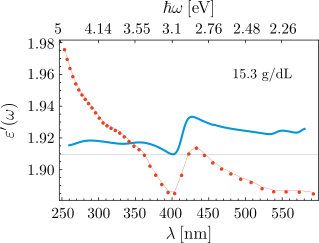
\includegraphics[width=0.47\textwidth]{../../Figuras/sskk15_0.pdf}\label{subfig:SSKK15}}}\hspace{0.1cm}
	\sidesubfloat[Second image]{\hspace{-0.6cm}{		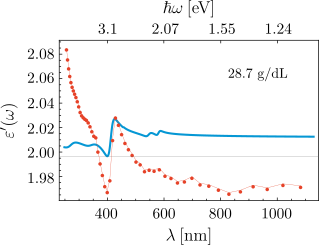
\includegraphics[width=0.47\textwidth]{../../Figuras/sskk28_0.pdf}\label{subfig:SSKK28}}}	\vspace{-0.2cm}
	\caption{Parte imaginaria de la función dieléctrica como función de la longitud de onda $\lambda$ (eje inferior) y la energía $\hbar\omega$ (eje superior). Se grafican datos experimentales representados por puntos rojos y el ajuste con lorenzianas con una línea azul continua para \textbf{a)} eritrocitos con una concentración de 15.3 g/dL, cuyos experimentales se obtuvieron de \cite{friebelDeterminationComplexRefractive2005a} y \textbf{b)} eritrocitos con una concentración de 28.7 g/dL, cuyos experimentales se obtuvieron de \cite{friebelModelFunctionCalculate2006}. En ambas las figuras las líneas grises verticales indican las frecuencias de resonancia asociadas a los osciladores de Lorentz empleados en el ajuste.}
	\label{fig:epsSSKK1}
\end{figure}
%
\begin{figure}[]
	\centering
	\includegraphics[width=0.45\textwidth]{../../Figuras/ajusteLorentzLegend.pdf}\\
	\sidesubfloat[Second image]{\hspace{-0.8cm}{		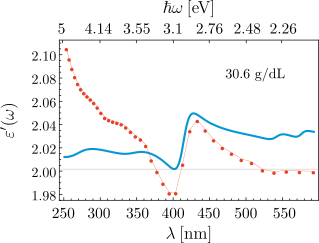
\includegraphics[width=0.47\textwidth]{../../Figuras/sskk30_0.pdf}\label{subfig:SSKK30}}}\hspace{0.1cm}
	\sidesubfloat[Second image]{\hspace{-0.6cm}{		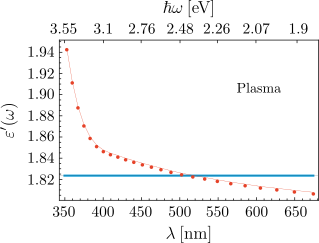
\includegraphics[width=0.47\textwidth]{../../Figuras/sskkPlasma_0.pdf}\label{subfig:SSKKPlasma}}} \vspace{-0.2cm}
	
	\caption{Parte imaginaria de la función dieléctrica como función de la longitud de onda $\lambda$ (eje inferior) y la energía $\hbar\omega$ (eje superior). Se grafican datos experimentales representados por puntos rojos y el ajuste con lorenzianas con una línea azul continua para \textbf{a)} eritrocitos con una concentración de 30.6 g/dL, cuyos experimentales se obtuvieron de \cite{friebelDeterminationComplexRefractive2005a} y \textbf{b)} plasma, cuyos experimentales se obtuvieron de \cite{meinkeOpticalPropertiesPlatelets2007a}. En ambas las figuras las líneas grises verticales indican las frecuencias de resonancia asociadas a los osciladores de Lorentz empleados en el ajuste.}
	\label{fig:epsSSKK2}
\end{figure}
%
\vspace{-0.5cm}

Para comparar la reconstrucción obtenida mediante SSKK con la reconstrucción basada en KK reportada en \cite{bosschaartLiteratureReviewNovel2014a}, se aplicaron las relaciones SSKK a los datos de la parte imaginaria del índice de refracción correspondientes a una CHCM de 28.7~g/dL, extraídos de \cite{friebelDeterminationComplexRefractive2005a}. Como punto de anclaje se empleó el valor experimental de la parte real del índice de refracción a una energía de 2.98~eV, también reportado en \cite{friebelDeterminationComplexRefractive2005a}. En la Fig.~\ref{fig:reconstru} se muestra la reconstrucción de la parte real del índice de refracción obtenida mediante SSKK (línea azul continua), junto con la reconstrucción obtenida mediante KK (línea azul oscuro continua) y los datos experimentales empleados para el punto de anclaje (puntos rojos). Se observa que el uso de SSKK no sólo asegura la coincidencia exacta en el punto de anclaje, sino que además reduce la desviación promedio respecto a los datos experimentales en todo el intervalo espectral considerado en aproximadamente un factor de tres, en comparación con la reconstrucción basada únicamente en KK.
%
\begin{figure}[h!]
	\centering
	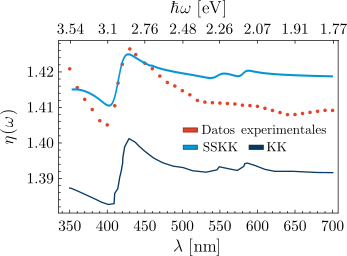
\includegraphics[width=8cm]{../../Figuras/Recontruccion.pdf}\vspace{-0.2cm}
	\caption{Parte real del índice de refracción de una CHCM de 28.7 g/dL en función de la longitud de onda $\lambda$ (eje inferior) y la energía $\hbar\omega$ (eje superior). Se grafican con puntos rojos los datos experimentales extraídos de \cite{friebelDeterminationComplexRefractive2005a} que se emplearon para comparar la reconstrucción y las reconstrucciones obtenidas mediante SSKK (línea azul claro continua) y mediante KK (línea azul oscuro continua) obtenida de  \cite{bosschaartLiteratureReviewNovel2014a}.}
	\label{fig:reconstru}
\end{figure}
%






